

\section{The Goswami Problem}

\label{sec:Goswami}

%\large{\bf Saltwater intrusion benchmark on laboratory-scale experiments}\\
%by Marc Walther and Jens-Olaf Delfs. \\ 
%\normalsize

\subsection{Definition}
This example shows density dependent groundwater flow under unconfined conditions. The benchmark is based on experimental and modelling data aquired by \textsc{Goswami et al, 2007} \cite{GosCle:2007}, who show a \textsc{Henry}-like (see \cite{PhDHenry:1960}) saltwater intrusion experiment using a laboratory-scale tank. 

\textsc{Goswami} showed three steady-state (SS-1, SS-2, SS-3), differing in the hydraulic gradient, and two transient (TS-1, TS-2) experiments, one advancing front condition (from the final states of experiments SS-1 to SS-2) and one receding front condition (SS-2 to SS-3) experiment, and concurrent simulations with \textsc{Seawat}. 

The model set-up will be as close as possible to the one used by \textsc{Goswami} exemplarily showing the simulations of SS-1 and TS-1 with \textsc{OpenGeoSys}.

\paragraph*{Method.} Modifying the Richards-Flow equation \cite{Ric:1931} with a linear approach as described by \textsc{Sugio et al, 1987} \cite{SugDes:1987} the hydraulic flow equation is solved for the unconfined flow. Additionally, the \textsc{Mass\_Transport} and \textsc{Richards\_Flow} processes are coupled via a density correlation as a function of concentration. 

%\begin{figure} [h!b]
% \centering 
% \includegraphics[width=0.5\textwidth] {H_US/figures/goswami_k_rel.eps}
% \caption{Examplary reduction function for relative permeabiltity $k_{rel}\left(p\right)$ depending on pressure $p$ after \textsc{Sugio et al, 1987} \cite{SugDes:1987}}
% \label{us:sugio_perm_redu}
%\end{figure}

\paragraph*{Boundary and initial conditions.} Boundary conditions are shown in figure \ref{dp:goswami_BC}: bottom and top horizontal boundaries are \textit{no-flow}, vertical right and left hand side boundaries are described via linear pressure gradients (including the appropriate densities of fresh water $\rho_f=1000kg\cdot m^{-3}$ or salt water $\rho_s=1026kg\cdot m^{-3}$), vertical right and left hand side boundary \textsc{Isochlor} concentrations $C_i$ are fresh water (i.e. $C_i=0$) and salt water (i.e. $C_i=1$), respectively.

For the SS-1 simulation, initial conditions are fresh water for the whole domain, i.e. a linear pressure gradient with $p_{\left(z=0.25m\right)}=0\mathrm{Pa}$ and $C_i=0$. 

For the TS-1 simulation, initial conditions are the hydraulic and mass transport steady state of SS-1.

\begin{figure} [h!]
 \centering 
 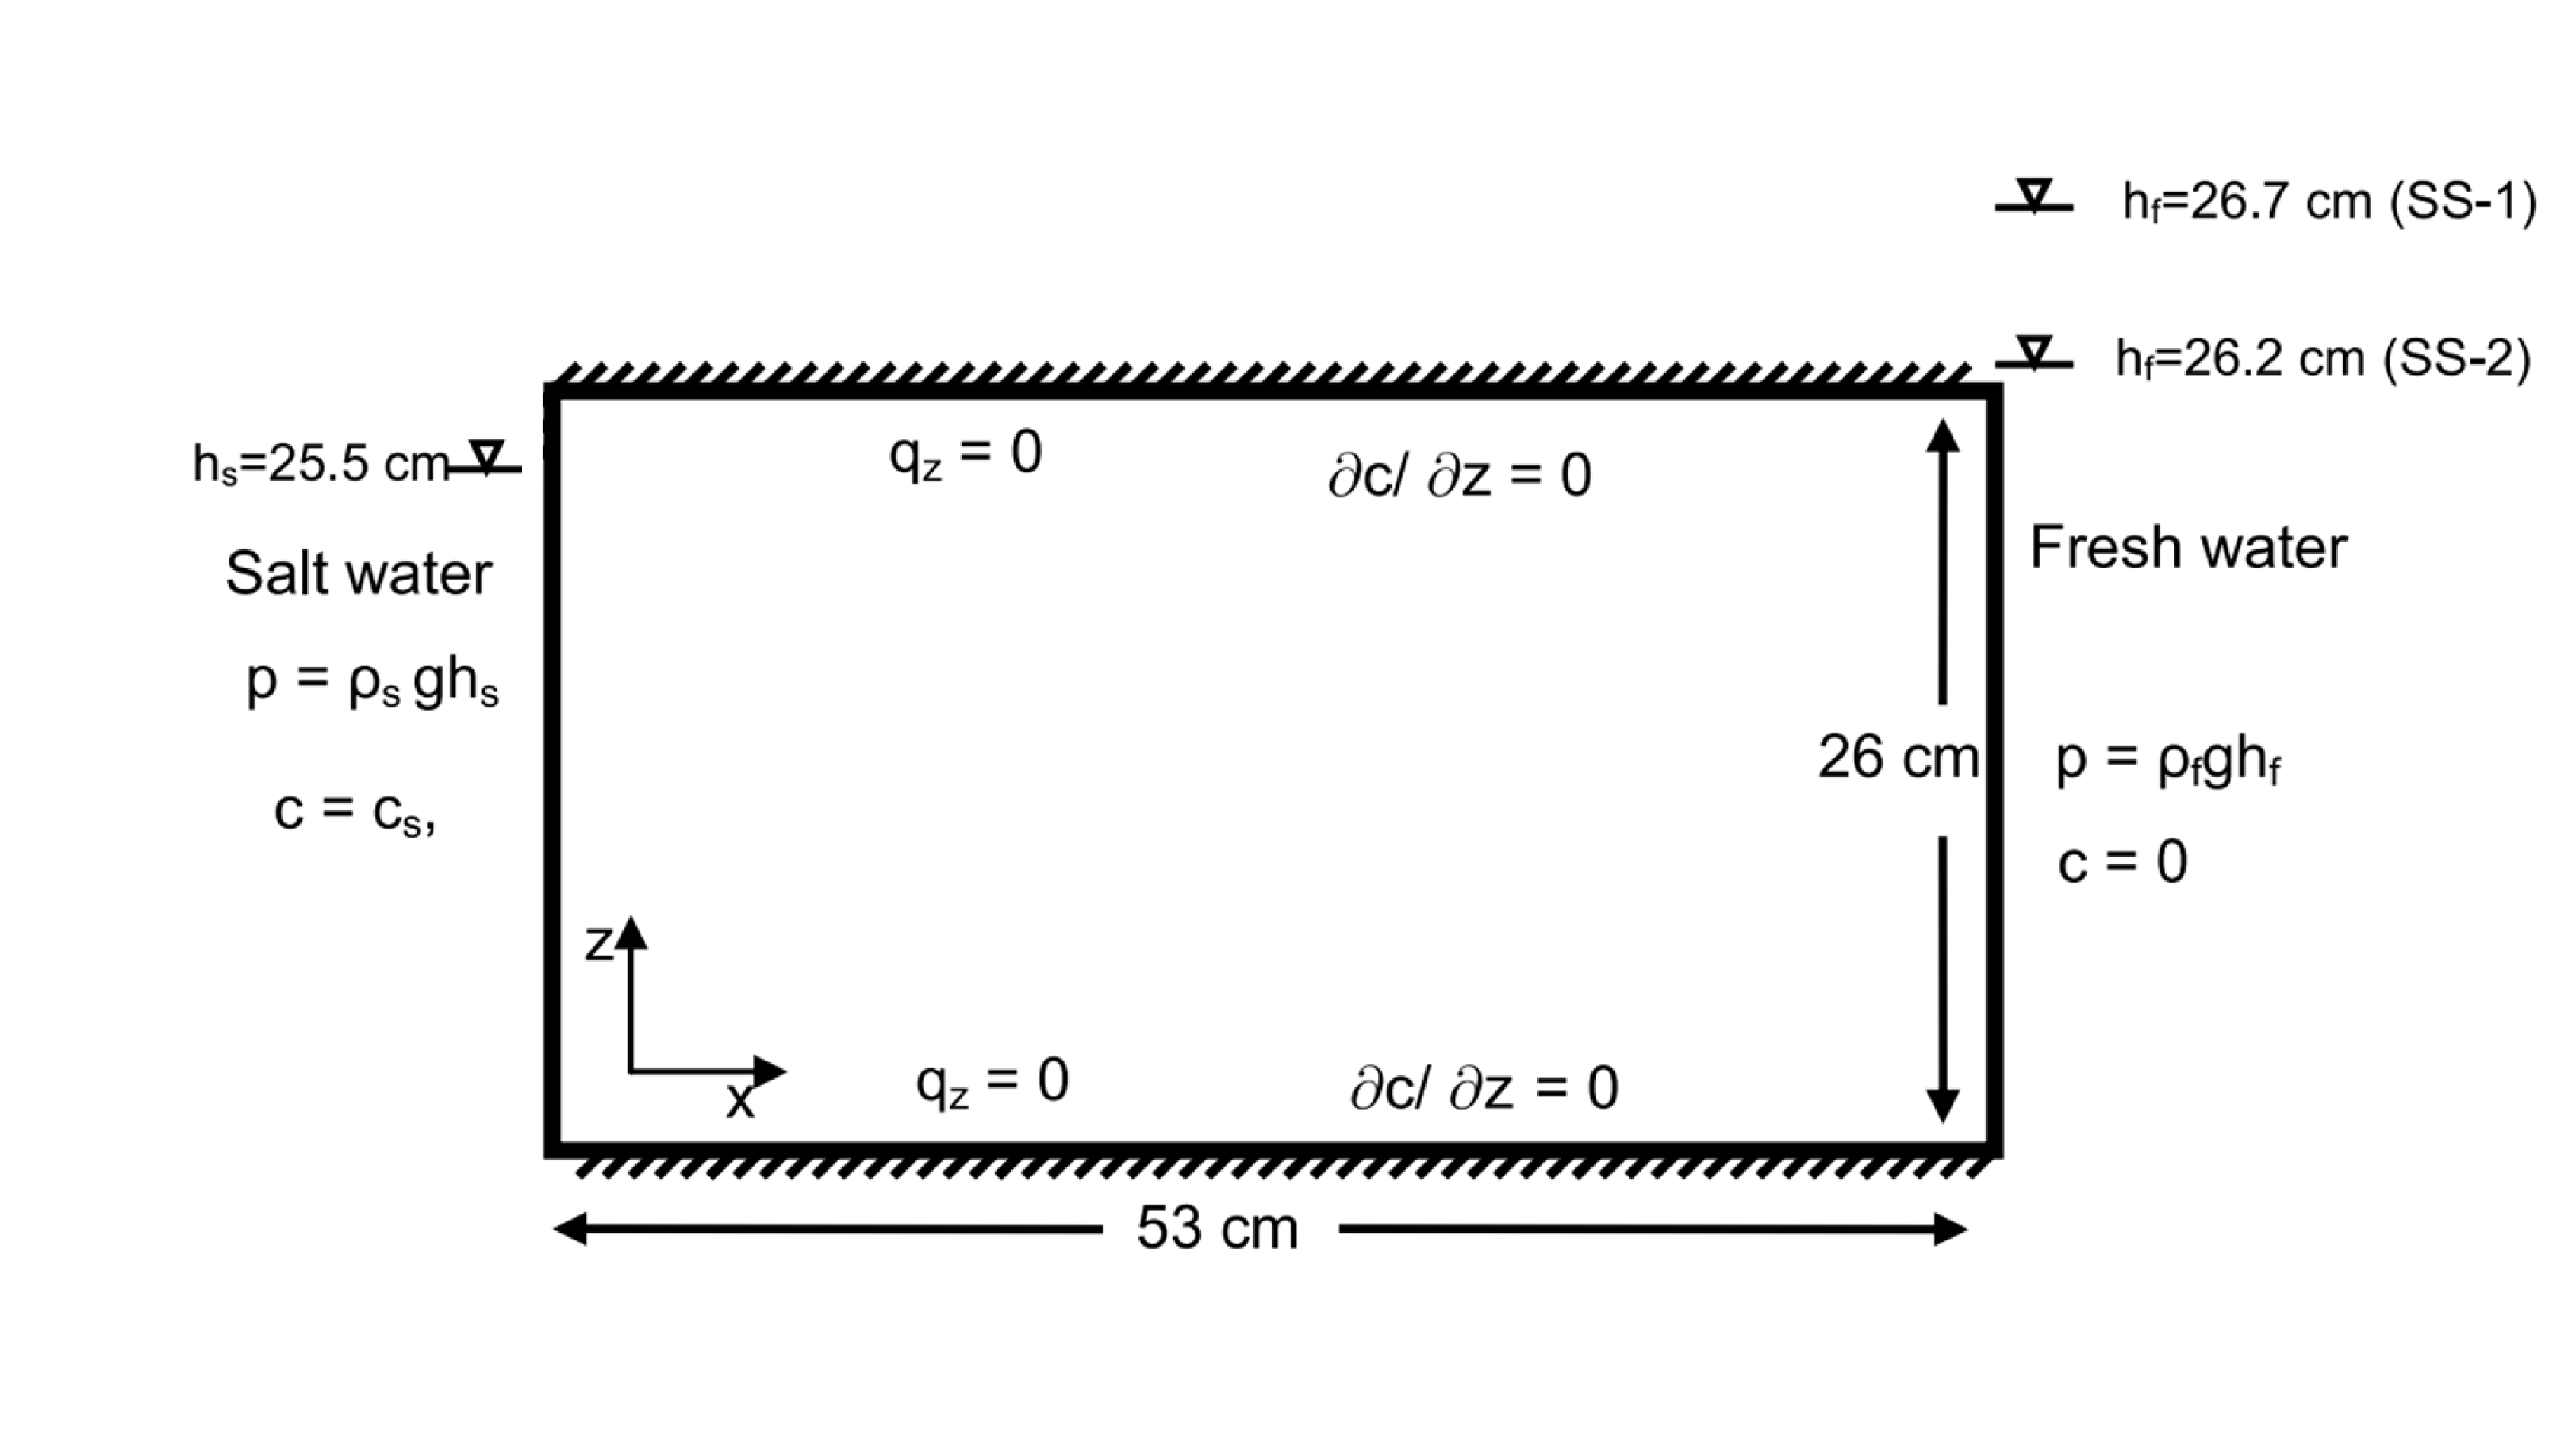
\includegraphics[width=0.85\textwidth] {PART_III/DDF/figures/goswami_bench_BC.eps}
 \caption{Model domain and boundary conditions after \textsc{Goswami et al, 2007} \cite{GosCle:2007}}
 \label{dp:goswami_BC}
\end{figure}

\paragraph*{Material properties.} The homogeneous, isotropic domain material equals a medium coarse sand. The corresponding parameters are listed in table \ref{dp:goswami_parameters}. %\textsc{Goswami} does not state any parameter value for specific storage for his transient simulations; here, it is set to zero, i.e. instant hydraulic response when changing the boundary conditions.

\textsc{\begin{table} [h!]
 \centering 
 \caption{Parameters of simulation}
 \label{dp:goswami_parameters}
 \begin{tabular}{ll}
 \toprule
 Parameter & Setting  \\ 
 \midrule
 Porosity    $[-]$           & $0.385$ \\
 Permeability $[m^2]$  &  $1.239\cdot 10^{-9}$ \\
 Reduced permeability $[m^2]$  & $0.0001$ \\
 Permeability reduction pressure $[Pa]$ & $-100$ \\
 \bottomrule
 \end{tabular}
\end{table}}

\paragraph*{Model domain, grid discretization.} The dimensions of the laboratory tank were $0.53$ x $0.26$ x $0.027 m^3$; following these measures, a 2D model domain was set up. The grid discretization was uniform with rectangular quad-elements sized $\Delta x = \Delta z = 5\cdot 10^{-4}m$. 

\paragraph*{Time stepping, Dispersivity, Diffusivity.} Time step was chosen to be $\Delta t = 10s$ up to a simulation time of $t_{final} = 4800s=80min$ (time until steady state of simulation); to the end of the simulation, time step size was increased up to $\Delta t = 160s$. 

Longitudinal dispersivity $\alpha_L$ was determined by \textsc{Goswami}'s laboratory experiments to $\alpha_L = 10^{-3}m$, transversal dispersivity $\alpha_T$ was assumed to be $\alpha_T = 0.1\cdot\alpha_L = 10^{-4}m$. 

Diffusion effects were neglected due to the highly advective flow regime.

\paragraph*{Stability.} Based on these model configurations, \textsc{Peclet} criterium is met within acceptable ranges with 
\begin{equation}
\mbox{Pe}=\frac{\Delta t\cdot v}{\Delta x} = \frac{10s\cdot 2\cdot 10^{-4}ms^{-1}}{5\cdot 10^{-3}m} = 0.4 < 1.
\end{equation}
However, \textsc{Courant} criterium is exceeded by its reglementations with 
\begin{equation}
\mbox{Co}=\frac{\Delta x}{\alpha} = \frac{5\cdot 10^{-3}m}{10^{-4}m} = 50 \nless 2,
\end{equation}
which causes some oscillations around the left side \textsc{Isochlor} boundary condition.% (comp. figure \ref{dp:goswami_comp_exp_SeaWat_OGS_dispersion_zone}).

\subsection{Results}
\paragraph*{Steady state.} Figure \ref{dp:goswami_ss-1_ogs} shows the \textsc{OpenGeoSys} simulation result of the steady-state scenario SS-1 and the typical circulation patterns of a saltwater intrusion, figure \ref{dp:goswami_comp_exp_SeaWat_OGS} shows the comparison of the experimental measurements with the modeling software outputs of SS-1 for \textsc{Seawat} and \textsc{OpenGeoSys}; the scenario simulations fit very well to the experimental observations. The slight deviations of both simulations may be due to the misfit of the \textsc{Courant} criterium, to inhomogeneities within the sand material, or to the measurement technique used to obtain the 0.5-\textsc{Isochlor} isolines, which was a simple visual observation of the dyed salt water. \textsc{Goswami} describes it as follows: \textit{``The color variations [...] indicate that the dispersion zone is relatively narrow and is estimated to be about $1 cm$ wide. Therefore the wedge delineation line [...] (which is assumed to be the 0.5 isochlor) has an error in the range of $\pm 0.5 cm$ [...]''}. As the dispersion zone was estimated to be about $1 cm$ wide an in such a way \textit{identified} 0.5-\textsc{Isochlor} isoline could very well also be a 0.1 or 0.9-\textsc{Isochlor} isoline. 

\textit{Note: Recently, an interesting work was done by this group concerning this issue, i.e. image analysis used for concentration measurements: see \cite{gos:2009}.}

%Comparing the simulated dispersion zone seen in figure \ref{dp:goswami_comp_exp_SeaWat_OGS_dispersion_zone}, \textsc{OpenGeoSys} simulationes show a slightly wider zone of dispersion.

In addition, tab. \ref{dp:goswami_flow_results} shows an overview of the right boundary's inflow from \textsc{Goswami}'s measured experimental data, the \textsc{Seawat} results and the equivalent values simulated with \textsc{OpenGeoSys}. Again, both simulation outputs resemble the measured experimental data within acceptable error limits.

\begin{table}
 \centering 
 \caption{Simulation results: right boundary influx $[cm^3\cdot s^{-1}]$}
 \label{dp:goswami_flow_results}
 \begin{tabular}{ll}
 \toprule
 Origin of value & SS-1 \\ %& SS-2 & SS-3 \\ 
 \midrule
 Experiment & 1.42 \\ %& 0.59 & 1.19 \\ 
 \textsc{Seawat} & 1.46 \\ %& 0.59 & 1.13 \\
 \textsc{OpenGeoSys} & 1.41 \\ %& 0.60 & 1.17 \\
 \bottomrule
 \end{tabular}
\end{table}

\paragraph*{Transient state.} 
Figure \ref{dp:goswami_comp_OGS_SeaWat_TS-1} depicts the comparison of the transient simulation of the experiment with both numerical models. While \textsc{Seawat} seems to fit the measurements quite well, \textsc{OpenGeoSys} shows slight differences; both results however, resemble the experimental data in an adequate way. 

\begin{figure}
 \centering 
 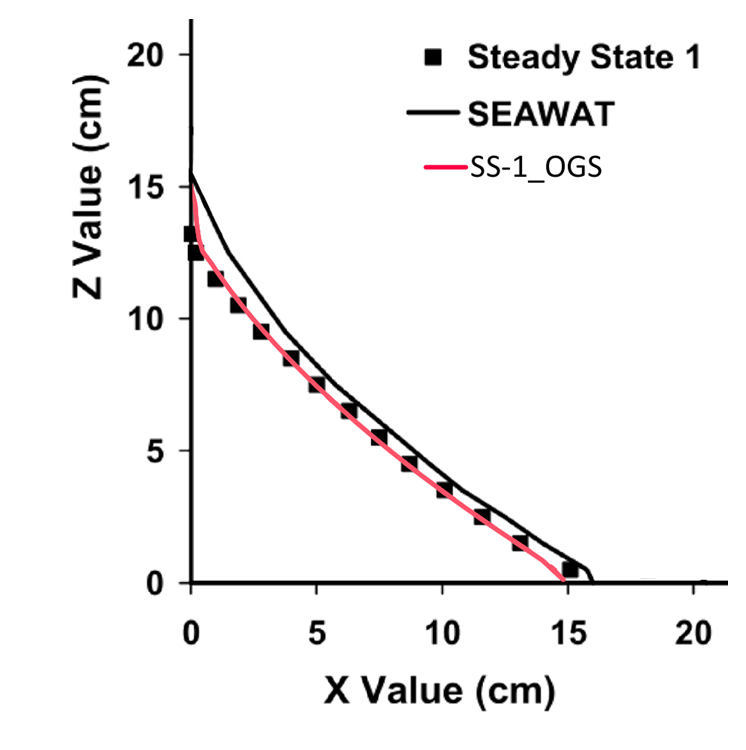
\includegraphics[width=0.65\textwidth] {PART_III/DDF/figures/goswami_comp_exp_OGS_SeaWat_SS-1.eps}	%goswami_comp_exp_SeaWat_OGS2
 \caption{Comparison of the 0.5-\textsc{Isochlor} concentration isolines of \textsc{Goswami}'s experimental data with his \textsc{Seawat} and the \textsc{OpenGeoSys} steady-state simulation}
 \label{dp:goswami_comp_exp_SeaWat_OGS}
\end{figure}

\begin{figure}
 \centering 
 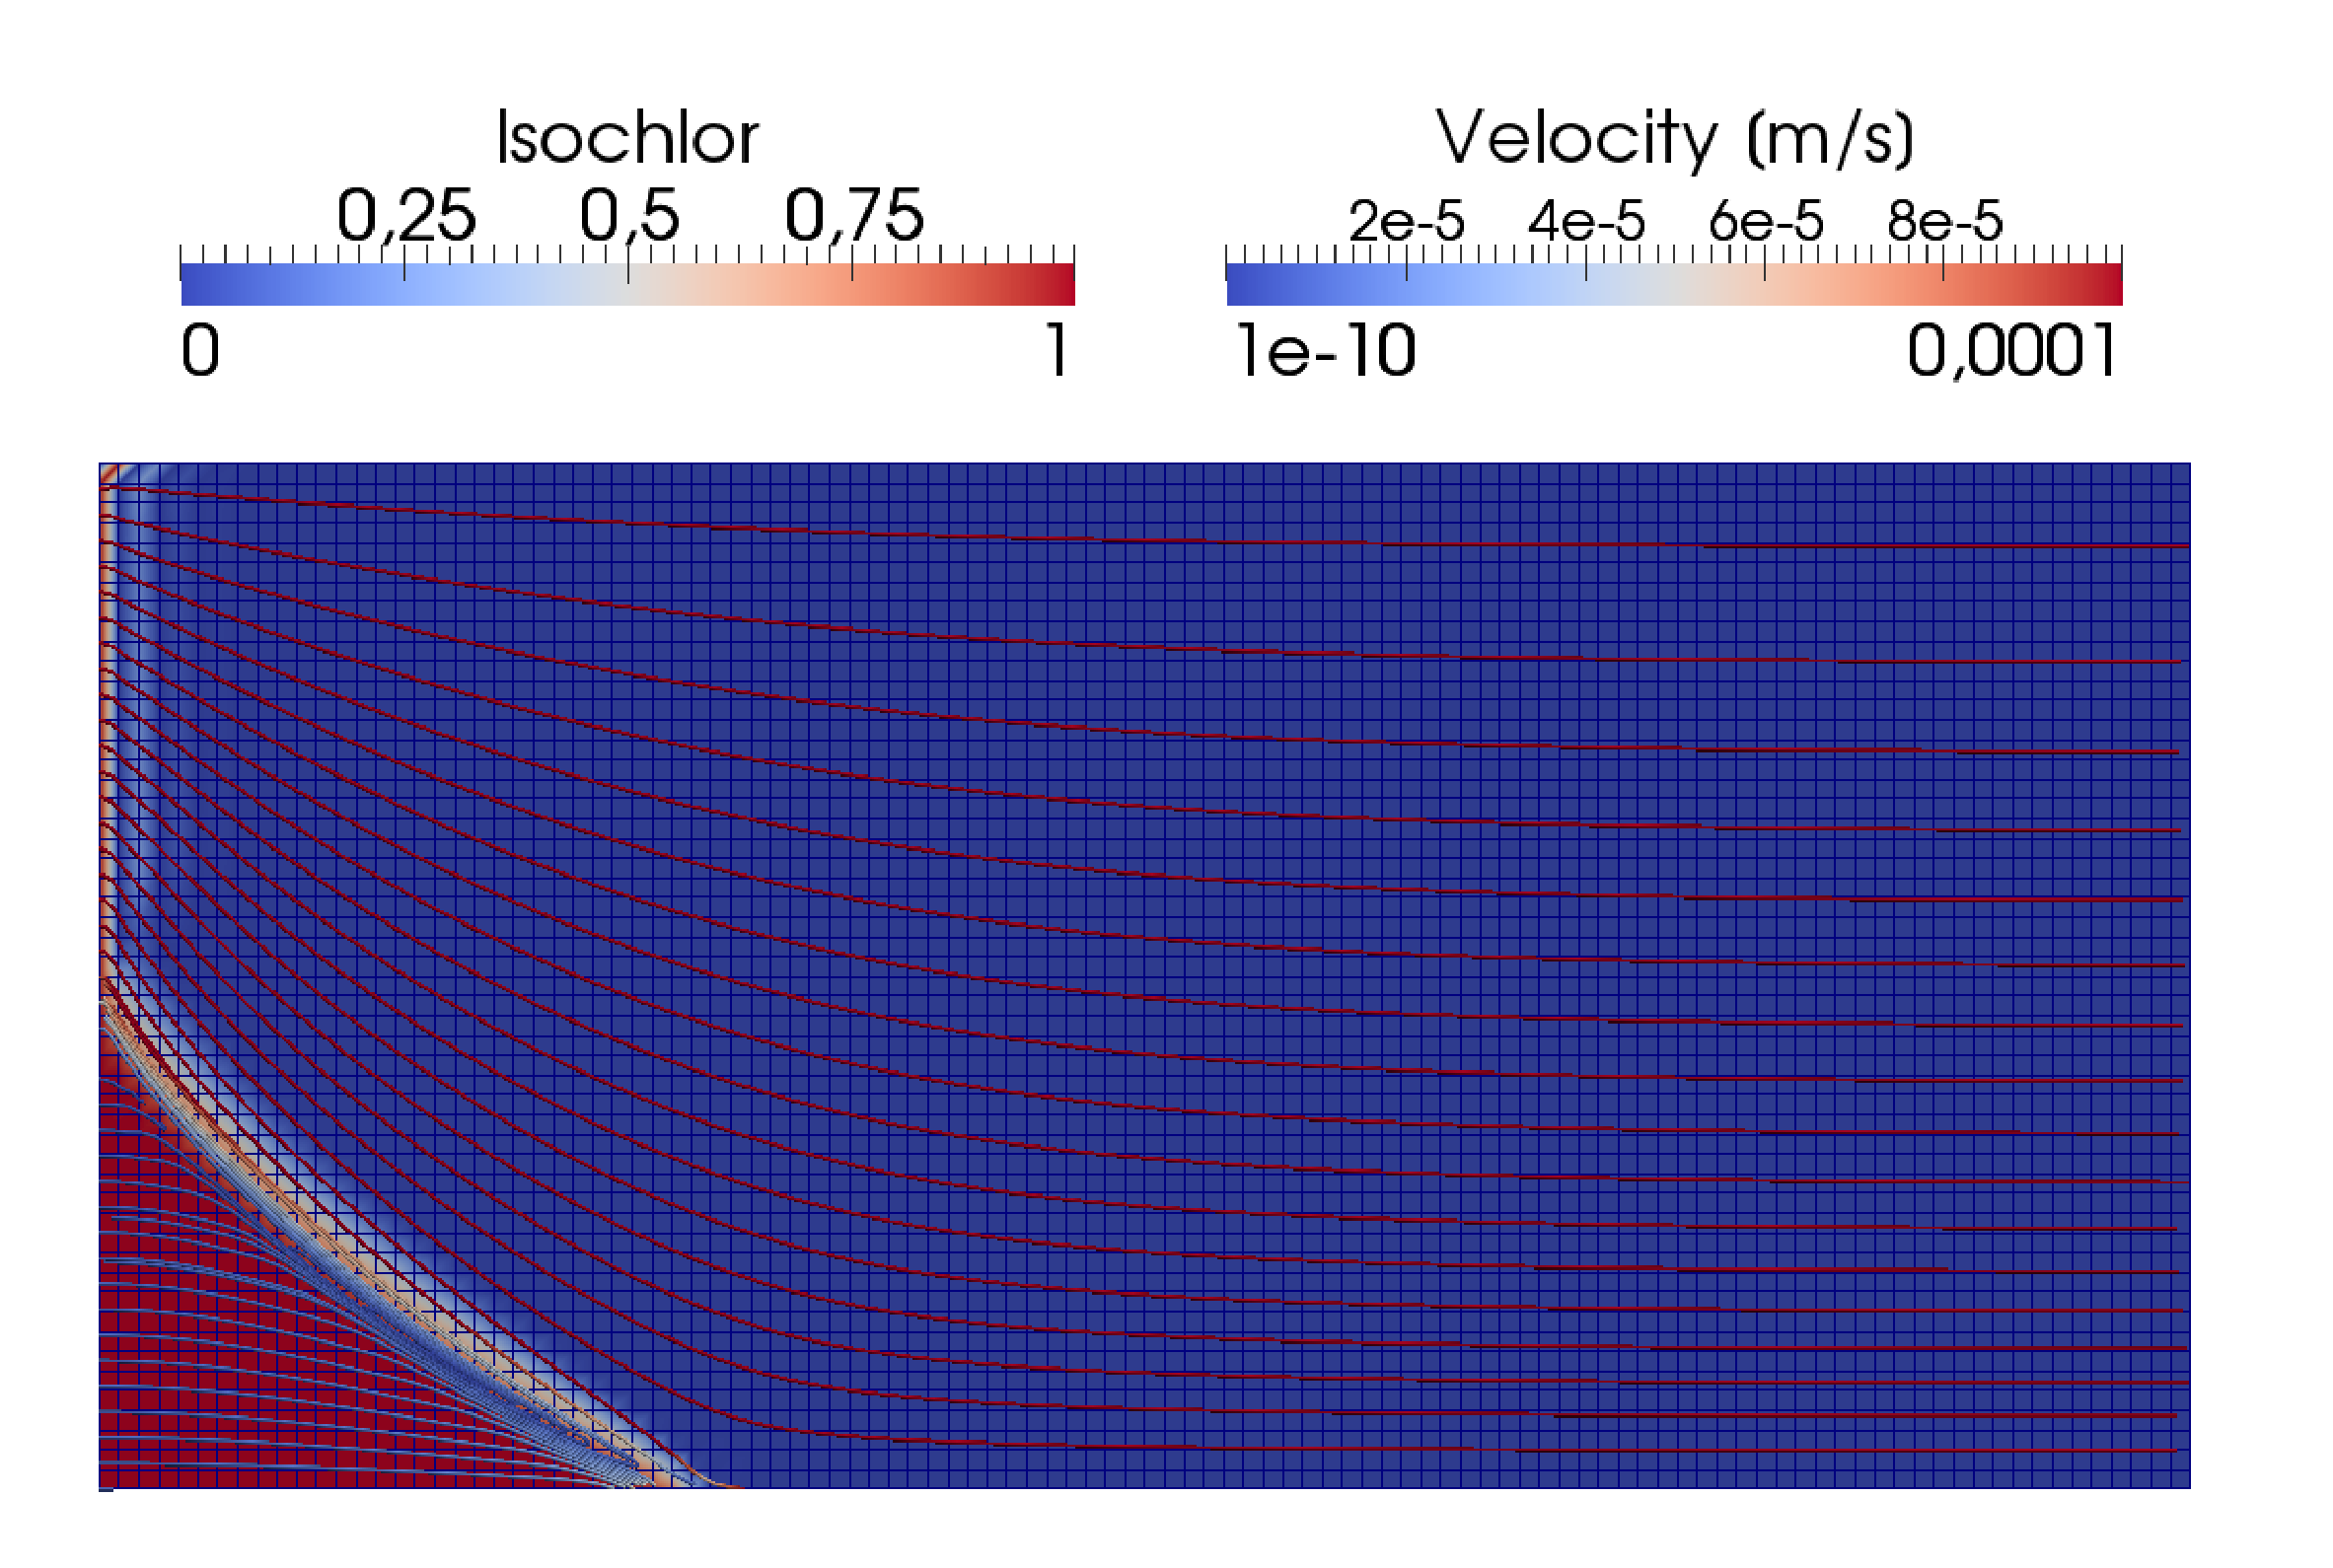
\includegraphics[width=0.8\textwidth] {PART_III/DDF/figures/goswami_flow_results.eps}
 \caption{\textsc{Isochlor}-concentration, flow field and grid resolution of the \textsc{OpenGeoSys} steady-state simulation SS-1}
 \label{dp:goswami_ss-1_ogs}
\end{figure}



%\begin{figure} 
% \centering 
% \includegraphics[width=0.85\textwidth] {PART_III/DDF/figures/goswami_comp_OGS_SeaWat_dispersion_zone.eps}
% \caption{Comparison of the dispersion zones showing 0.1, 0.5 and 0.9-\textsc{Isochlor} concentration isolines of \textsc{Goswami}'s experimental data, his \textsc{Seawat} (black) and the \textsc{OpenGeoSys} (blue) simulations}
% \label{dp:goswami_comp_exp_SeaWat_OGS_dispersion_zone}
%\end{figure}


\begin{figure}
 \centering 
 \includegraphics[width=0.9\textwidth] {PART_III/DDF/figures/goswami_comp_OGS_SeaWat_TS-1.eps}
 \caption{Comparison of the 0.5-\textsc{Isochlor} concentration isolines of \textsc{Goswami}'s experimental data with his \textsc{Seawat} and the \textsc{OpenGeoSys} transient simulation TS-1}
 \label{dp:goswami_comp_OGS_SeaWat_TS-1}
\end{figure}

%\begin{figure} 
% \centering 
% \includegraphics[width=0.85\textwidth] {PART_III/DDF/figures/goswami_comp_OGS_SeaWat_TS-2.eps}
% \caption{Comparison of the 0.5-\textsc{Isochlor} concentration isolines of \textsc{Goswami}'s experimental data with his \textsc{Seawat} and the \textsc{OpenGeoSys} transient simulation TS-2}
% \label{dp:goswami_comp_OGS_SeaWat_TS-2}
%\end{figure}


%\clearpage
%\subsubsection*{Benchmark deposit} 
%\begin{table} [h!]
%\begin{tabular}{|l|l|l|} 
%  \hline
%  Benchmark & Problem type & Path in benchmark deposit \\
%  \hline
%  \textit{HM} & H & benchmarks/h\_us/Goswami/ \\
%  \hline
%\end{tabular}
%\end{table}